\documentclass{article}

\usepackage{helvet}
\renewcommand{\familydefault}{\sfdefault}
\usepackage{eurosym}

\usepackage{graphicx} % allows for working with images
\DeclareGraphicsExtensions{.pdf,.png,.jpeg,.jpg,.gif} % configures latex to look for the following image extensions

\usepackage{tabularx}
\usepackage[table]{xcolor}

% fix for \rowcolors in {tabularx}, see https://tex.stackexchange.com/a/297357/4918
\newcounter{tblerows}
\expandafter\let\csname c@tblerows\endcsname\rownum
\usepackage{booktabs}

\begin{document}
\pagenumbering{gobble}


\section*{SEMS Information}

\subsection*{Membership Dues}
Thanks for your application to join the South East Makerspace. Once your membership has been approved, you will be provided with a \textbf{membership reference number}. This number must be used as the transfer reference when making your monthly membership payments to allow you to be correctly identified for our records.

The monthly membership fees is \textbf{\euro20} and is paid for the month in advance. Currently the only method of paying membership dues is through a bank transfer. We are investigating the possibility of using a service such as paypal in the future. The details for the account to make payment to are:

\begin{itemize}
\item IBAN: IE78 AIBK 93411914330037
\item BIK: AIBKIE2D
\end{itemize}


\subsection*{Meetings}
Every Tuesday between 7pm and 9pm, SEMS runs the Mad Maker event where you will find members in the space working on different projects or just having a chat. We're open to the public during these hours, if you want to pop down and say hi you are more than welcome!


\subsection*{Website + Wiki}
Wiki accounts are created for new members as part of the signup process. The wiki is used as a collaborative document to store meeting minutes, projects, admin documents and various other things for the space. Feel free to contribute, if you need any help using the wiki feel free to ask any member for help. We would suggest you create a profile on our members page to introduce yourself to the group \textit{http://wiki.southeastmakerspace.org/doku.php?id=member-pages}.


\subsection*{Mailing List}
SEMS also operates two mailing lists which we use to keep members informed. The general list is a public list used to communicate details such as next meetings and any public workshops which are planned. The members list is used for communication within the makerspace, use this to send a mail to the entire group. New members are signed up for both as part of the process, so please be sure to provide the correct email address on the membership form.


\subsection*{Social Media}
We also have a social media presence on several platforms which can you
follow/like to keep informed:

\begin{itemize}
\item Facebook https://www.facebook.com/SouthEastMakerSpace
\item Twitter https://twitter.com/SEMakerSpace
\item Google+ https://plus.google.com/u/0/108025738894009906004/posts
\end{itemize}


\subsection*{Address and Phone}

%
\begin{figure}[ht]
	\centering
	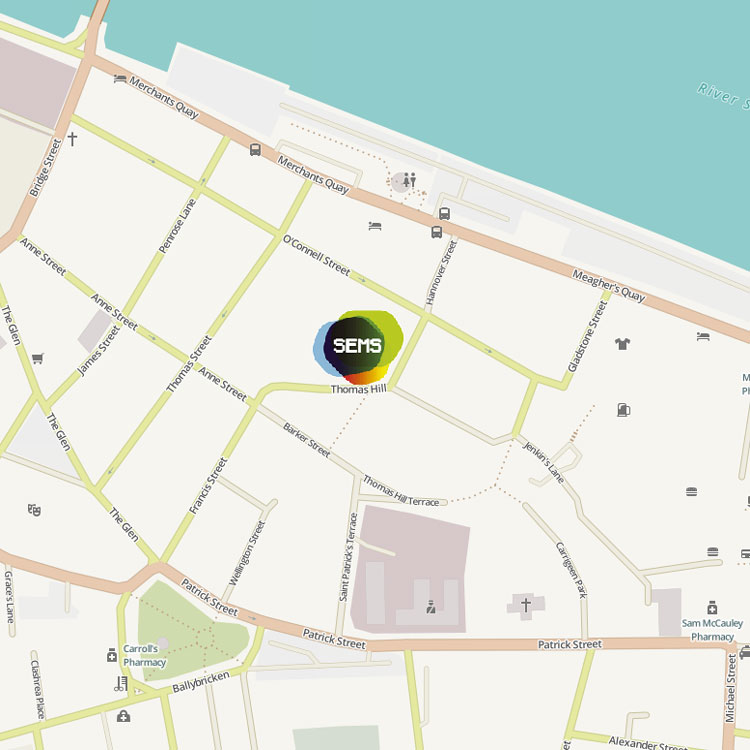
\includegraphics[width=9cm]{sems_local_map_750_750}
	\caption{SEMS Location}
	\label{fig:sems_location}
\end{figure}
%


\begin{verbatim}
SEMS
Old Printworks
Thomas Hill
Waterford City
WATERFORD
X91 TW63
Email: info@southeastmakerspace.org
Phone Number: +353 89 422 5909
\end{verbatim} \par

\section*{SEMS Locking up Checklist}

\subsection*{Important}
The following checklist \textbf{must} be performed by members of the South East Makerspace before closing the space down.


\begin{table}[h]
	\centering
	\caption{Closing up checklist} 
	\label{tab:checklist}
	\rowcolors{2}{}{black!10}
	\begin{tabularx}{.9\textwidth}{XX}
		\toprule
		\textbf{Task} & \textbf{Information} \\ 
		\midrule
		Turn off all heaters & Wall mounted electric heaters must be first switched off using their power cords, then switched off at the wall. The portable electric in snug must be switched off using the onboard switches, then switched off at the wall also. \textbf{purple} dots on map. \\ 
		Unplug or switch off all sockets & \textbf{red} dots on map. Do not switch off the fridge \\ 
		Shut off the water & \textbf{blue} dot on map. This is potentially more important in the Winter months \\ 
		Ensure all doors are locked (including cabinets) & \textbf{green} dots on map \\ 
		Shut off all the lights & \textbf{yellow} dots on map \\ 
		\bottomrule
	\end{tabularx}
\end{table}

%
\begin{figure}[ht]
	\centering
	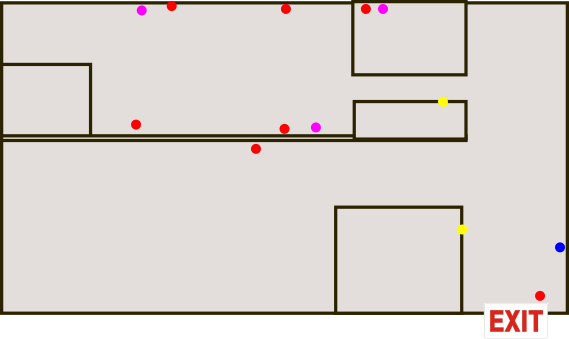
\includegraphics[width=9cm]{Sems}
	\caption{SEMS Interior Map}
	\label{fig:sems_map}
\end{figure}
%

\end{document}
